\documentclass[11pt]{article}
\usepackage[utf8]{inputenc}
\usepackage[spanish]{babel}
\usepackage[margin=2.2cm]{geometry}
\usepackage{tikz}
\usetikzlibrary{shapes,arrows.meta,positioning,calc,fit,backgrounds}
\usepackage{longtable}
\usepackage{booktabs}
\usepackage{array}
\usepackage{hyperref}
\usepackage{enumitem}
\usepackage{titlesec}
\usepackage{xcolor}

\titleformat{\section}{\large\bfseries}{P\thesection.}{0.4em}{}
\renewcommand{\thesection}{\arabic{section}}

\begin{document}

% ============ CARÁTULA ============
\begin{titlepage}
\centering


{\large UNIVERSIDAD TÉCNICA ESTATAL DE QUEVEDO\par}
\vspace{0.1cm}
{\large FACULTAD DE CIENCIAS DE LA COMPUTACIÓN\par}
\vspace{0.1cm}
{\large CARRERA DE INGENIERÍA DE SOFTWARE, 4TO NIVEL\par}



\rule{\linewidth}{0.6pt}\par


{\Large\bfseries PRUEBA PRÁCTICA --- UNIDAD IV\par}
{\large Validación, Gestión, Herramientas y Estándares de Requisitos\par}
{\normalsize Caso: Sistema de Gestión de Pedidos\par}


\rule{\linewidth}{0.6pt}\par


\begin{tabular}{ll}
\textbf{Asignatura:} & Ingeniería de Requerimientos \\ [1pt]
\textbf{Estudiante:} & Kleber Obed Crespo Espinoza \\ [3pt]
\textbf{Docente:} & Ing. Gleiston Guerrero, Mg. \\
\end{tabular}



\vspace{0.10cm}

{\bfseries Repositorio:} \\
\url{https://github.com/kcrespoe/Crespo-ISR401-Prueba-U4} 


\vspace{0.2cm}


% ============ CAPTURAS ============
\begin{minipage}{0.95\textwidth}
\centering
\fbox{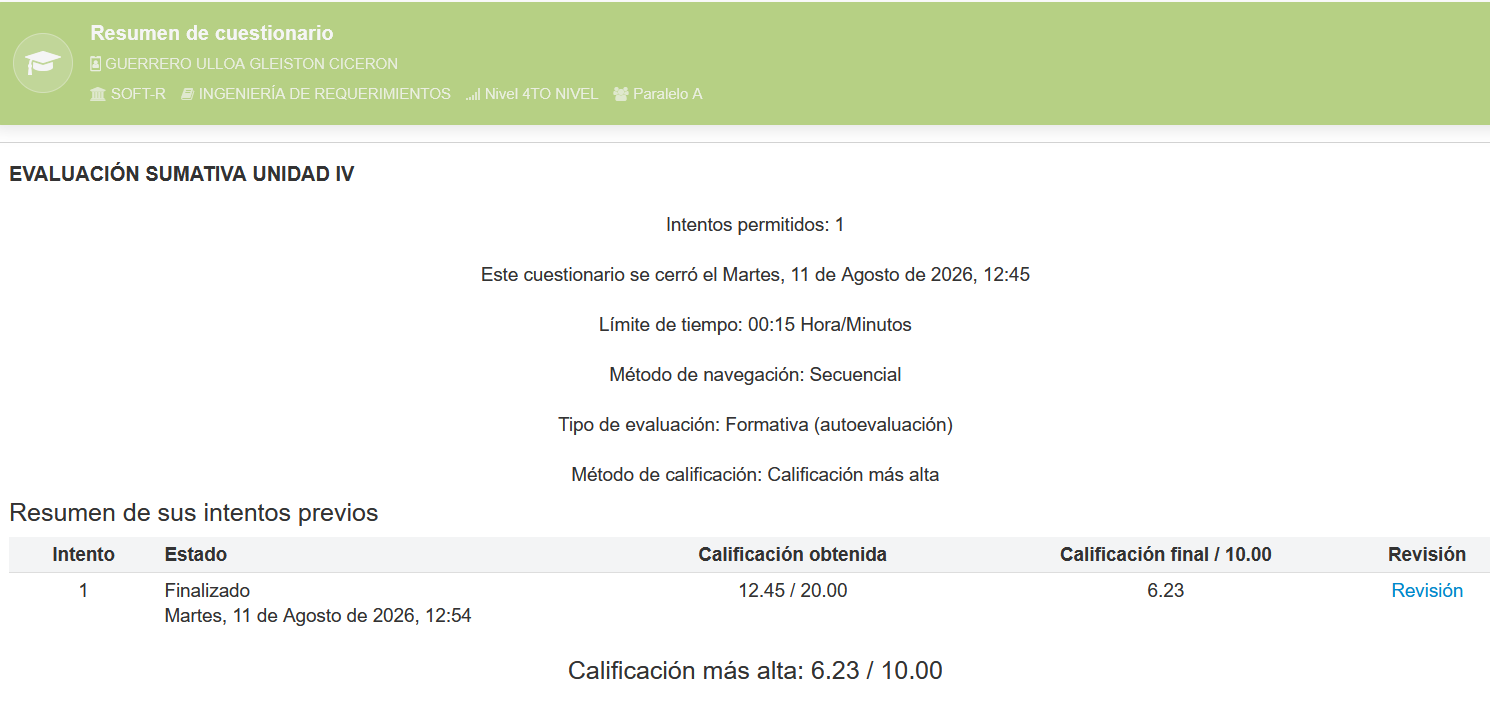
\includegraphics[
width=\textwidth,
height=0.35\textheight,
keepaspectratio
]{captura_resumen.png}}
\vspace{1pt}
{\small\itshape Fig. 1: Resumen\par}
\vspace{0.15cm}
\fbox{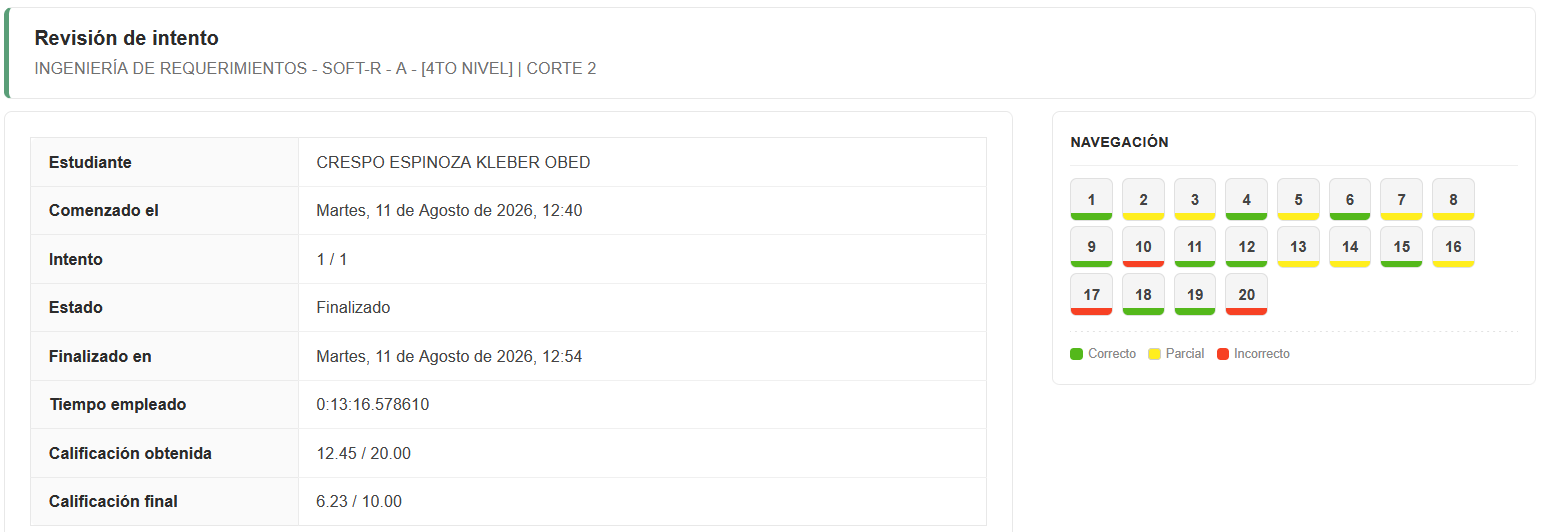
\includegraphics[
width=\textwidth,
height=0.8\textheight,
keepaspectratio
]{captura_evaluacion.png}}
\vspace{1pt}
{\small\itshape Fig. 2: Resultado de la evaluación\par}
\end{minipage}
\vfill


{\normalsize Quevedo -- Ecuador\par}
{\normalsize \the\year\par}

\end{titlepage}

% ============ FIN CARÁTULA ============

{\centering\Large\bfseries Sistema de Gestión de Pedidos --- Respuestas de referencia (P1--P10)\par}
\vspace{0.3cm}

\section{Modelo de datos --- Diagrama de clases UML}

\begin{center}
\begin{tikzpicture}[
class/.style={
    draw,
    rectangle,
    align=left,
    text width=4.0cm,
    font=\scriptsize,
    inner sep=4pt
},
every node/.style={font=\scriptsize}
]

\node[class] (cliente) at (0,3.4) {
\textbf{Cliente}\\
\hrulefill\\
-- \underline{cedulaRuc} : String\\
-- nombre : String\\
-- correo : String\\
\hrulefill\\
+ realizarPedido(p: Pedido) : void
};

\node[class] (pedido) at (5.9,3.4) {
\textbf{Pedido}\\
\hrulefill\\
-- \underline{idPedido} : String\\
-- fecha : Date\\
-- total : Decimal\\
-- estado : EstadoPedido\\
\hrulefill\\
+ calcularTotal() : Decimal\\
+ confirmar() : void\\
+ anular() : void\\
+ notificarFaltante() : void
};

\node[class] (producto) at (11.8,3.4) {
\textbf{Producto}\\
\hrulefill\\
-- \underline{codigo} : String\\
-- descripcion : String\\
-- precio : Decimal\\
-- stock : Integer\\
\hrulefill\\
+ verificarStock(c: Integer) : Boolean
};

\node[class] (linea) at (5.9,-1.1) {
\textbf{LineaPedido}\\
\hrulefill\\
-- cantidad : Integer\\
-- precioUnitario : Decimal\\
\hrulefill\\
+ subtotal() : Decimal
};

% Cliente -- Pedido
\draw[-] (cliente) -- (pedido)
    node[midway, above=2pt, font=\tiny] {realiza};

\node[font=\tiny] at ($(cliente.east)+(0.3,-0.22)$) {1};
\node[font=\tiny] at ($(pedido.west)+(-0.35,-0.22)$) {0..*};

% Pedido -- LineaPedido
\draw[-] (pedido.south) -- (linea.north)
    node[pos=0.65, right=1pt, font=\tiny] {contiene};

\node[font=\tiny] at ($(pedido.south)+(-0.25,-0.15)$) {1};
\node[font=\tiny] at ($(linea.north)+(-0.35,0.15)$) {1..*};

% LineaPedido -- Producto
\draw[-] (linea.east) -| ($(producto.south)+(0,0)$);

\node[font=\tiny] at ($(linea.east)+(0.35,0.18)$) {0..*};
\node[font=\tiny] at ($(producto.south)+(0.3,-0.15)$) {1};
\node[font=\tiny] at (9.5,-1.4) {referencia};

\end{tikzpicture}
\end{center}


\section{Modelo funcional --- Diagrama de actividades ``Registrar pedido''}

\begin{center}
\begin{tikzpicture}[
  node distance=1.1cm,
  act/.style={draw, rectangle, rounded corners, minimum width=4.6cm, minimum height=0.9cm, align=center, font=\scriptsize},
  dec/.style={draw, diamond, aspect=2.2, align=center, font=\scriptsize, inner sep=1pt},
  ini/.style={draw, circle, fill=black, minimum size=0.28cm},
  fin/.style={draw, circle, fill=black, minimum size=0.28cm}
]
\node[ini] (ini) {};
\node[act, below=of ini] (a1) {Cliente: ingresa datos del pedido};
\node[dec, below=of a1] (dec) {¿Stock\\ disponible?};
\node[act, below left=1.2cm and -0.3cm of dec] (a2) {Sistema: confirma pedido};
\node[act, below right=1.2cm and -0.3cm of dec] (a3) {Sistema: notifica faltante};
\node[fin, below=2.6cm of dec] (fin) {};

\draw[-{Latex}] (ini) -- (a1);
\draw[-{Latex}] (a1) -- (dec);
\draw[-{Latex}] (dec) -| node[near start, above, font=\tiny]{Sí} (a2);
\draw[-{Latex}] (dec) -| node[near start, above, font=\tiny]{No} (a3);
\draw[-{Latex}] (a2) |- (fin);
\draw[-{Latex}] (a3) |- (fin);
\end{tikzpicture}
\end{center}


\section{Modelo de comportamiento --- Máquina de estados de Pedido}

\begin{center}
\begin{tikzpicture}[
  st/.style={draw, rounded corners, minimum width=2.2cm, minimum height=0.8cm, align=center, font=\scriptsize},
  ini/.style={draw, circle, fill=black, minimum size=0.25cm},
  fin/.style={draw, circle, fill=black, minimum size=0.25cm},
  lbl/.style={font=\tiny, align=center}
]
\node[ini] (ini) at (0,0) {};
\node[st] (reg) at (2.3,0) {Registrado};
\node[st, dashed, minimum width=7.6cm, minimum height=2.6cm] (super) at (8.7,0) {};
\node[font=\tiny, above] at (8.7,1.35) {EnProceso};
\node[st] (conf) at (6.6,0) {Confirmado};
\node[st] (env) at (10.4,0) {Enviado};
\node[st] (ent) at (14.2,0) {Entregado};
\node[fin] (finent) at (16.3,0) {};
\node[st] (canc) at (8.7,-2.7) {Cancelado};
\node[fin] (fincanc) at (8.7,-4.0) {};

\draw[-{Latex}] (ini) -- (reg);
\draw[-{Latex}] (reg) -- (conf) node[lbl, pos=0.5, above=2pt] {confirmar()\\ {[}stock OK{]}};
\draw[-{Latex}] (conf) -- (env) node[lbl, pos=0.5, above=2pt] {despachar()};
\draw[-{Latex}] (env) -- (ent) node[lbl, pos=0.5, above=2pt] {entregar()};
\draw[-{Latex}] (ent) -- (finent);
\draw[-{Latex}] (reg) -- (canc) node[lbl, pos=0.35, left=1pt] {anular()};
\draw[-{Latex}] (super.south) -- (canc) node[lbl, pos=0.45, right=1pt] {anular()\\ {[}no entregado{]}};
\draw[-{Latex}] (canc) -- (fincanc);
\end{tikzpicture}
\end{center}

\section{Consistencia entre las tres perspectivas}

\begin{center}
\small
\begin{tabular}{p{3cm}p{5cm}p{4.5cm}}
\toprule
\textbf{Evento (P3)} & \textbf{Función/Acción (P2)} & \textbf{Entidad/Atributo (P1)} \\
\midrule
confirmar() & ``Sistema: confirma pedido'' & Pedido.estado \\
anular() & \centering{-} & Pedido.estado \\
despachar() & \centering{-} & Pedido.estado \\
entregar() & \centering{-} & Pedido.estado \\
\bottomrule
\end{tabular}
\end{center}

\textbf{Inconsistencia detectada:} la acción ``Sistema: notifica faltante'' (P2) no tenía una operación equivalente en el diagrama de clases (P1).
\textbf{Corrección aplicada:} se agregó la operación \texttt{notificarFaltante(): void} a la clase \texttt{Pedido} (ya incluida en el diagrama de P1).

\section{Especificación de requisitos con esquema de atributos}

\begin{center}
\small
\begin{tabular}{p{1.3cm}p{6.3cm}p{1.2cm}p{1.4cm}p{1.6cm}}
\toprule
\textbf{ID} & \textbf{Requisito} & \textbf{Prior.} & \textbf{Fuente} & \textbf{Verif.} \\
\midrule
RF-01 & El sistema debe confirmar un pedido solo cuando exista stock suficiente del producto solicitado. & Alta & Caso §2 & Prueba funcional \\
RF-02 & El sistema debe permitir anular un pedido confirmado mientras no haya sido entregado. & Media & Caso §2 & Prueba funcional \\
RNF-01 & \emph{(Eficiencia de desempeño)} El sistema debe registrar un pedido en menos de 3 s con 100 usuarios concurrentes. & Media & Negocio & Prueba de rendimiento \\
RNF-02 & \emph{(Seguridad)} Los datos personales del cliente deben cifrarse (AES-256) en reposo y en tránsito, accesibles solo con autenticación. & Alta & Protección de datos & Auditoría de seguridad \\
\bottomrule
\end{tabular}
\end{center}
Todos: Estado = Propuesto; Estabilidad = Estable; Versión = 1.0 (RF-02 evoluciona a 1.1 en P10).

\section{Priorización MoSCoW}

\begin{center}
\small
\begin{tabular}{p{1.3cm}p{1.6cm}p{9.5cm}}
\toprule
\textbf{ID} & \textbf{Categoría} & \textbf{Justificación} \\
\midrule
RF-01 & \textbf{Must} & Núcleo funcional; sin verificación de stock el sistema no puede operar. \\
RNF-02 & \textbf{Must} & Obligación legal de protección de datos personales. \\
RF-02 & \textbf{Should} & Importante para el ciclo de vida, pero el sistema opera sin anulación inmediata. \\
RNF-01 & \textbf{Could} & Mejora deseable de rendimiento; no bloquea la operación básica. \\
\bottomrule
\end{tabular}
\end{center}

\section{Validación por inspección (ISO/IEC/IEEE 29148)}

\textbf{Defectos detectados (sin corregir):}
\begin{enumerate}[itemsep=1pt]
  \item RF-01 (versión original) --- \emph{no singular}: mezclaba ``registrar'' y ``verificar stock'' en un solo enunciado.
  \item RNF-02 (versión original) --- \emph{no verificable}: no definía mecanismo ni métrica medible para la autenticación.
\end{enumerate}

\textbf{Retrabajo (requisitos corregidos):}
\begin{itemize}[itemsep=1pt]
  \item RF-01: ``El sistema debe confirmar un pedido solo cuando exista stock suficiente del producto solicitado.'' (singular y verificable).
  \item RNF-02: ``Los datos personales del cliente deben cifrarse con AES-256 en reposo y en tránsito, verificable mediante auditoría de seguridad con 0 hallazgos críticos.''
\end{itemize}

\section{Pruebas de aceptación trazadas}

\begin{center}
\small
\begin{tabular}{p{1.1cm}p{2cm}p{3.7cm}p{3.7cm}p{0.9cm}}
\toprule
\textbf{ID} & \textbf{Tipo} & \textbf{Entradas} & \textbf{Criterio de éxito} & \textbf{Traza} \\
\midrule
PA-01 & Funcional & Producto P001, stock=5, cantidad=3 & Pedido confirmado; stock=2 & RF-01 \\
PA-02 & Funcional & Pedido confirmado no entregado; anular & Estado pasa a Cancelado & RF-02 \\
PA-03 & No func. (rendimiento) & 100 solicitudes concurrentes & 95\% de respuestas $<3$s & RNF-01 \\
PA-04 & No func. (seguridad) & Acceso no autenticado a datos del cliente & Acceso denegado; datos cifrados & RNF-02 \\
\bottomrule
\end{tabular}
\end{center}

\section{Matriz de trazabilidad}

\begin{center}
\scriptsize
\begin{tabular}{p{1cm}p{2.2cm}p{3.1cm}p{1.1cm}p{2.6cm}p{1.6cm}}
\toprule
\textbf{ID} & \textbf{Fuente (atrás)} & \textbf{Modelo (adelante)} & \textbf{Prueba} & \textbf{Dep. horizontal} & \textbf{¿Huérfano?} \\
\midrule
RF-01 & Caso §2 & P1 (Pedido/Producto), P2, P3 (Confirmado) & PA-01 & Depende de RNF-02 & No \\
RF-02 & Caso §2 & P1 (Pedido), P3 (Cancelado) & PA-02 & Depende de RF-01 & No \\
RNF-01 & Negocio ``rapidez'' & P2 (proceso registrar) & PA-03 & --- & No \\
RNF-02 & Protección de datos & P1 (clase Cliente) & PA-04 & --- & \textbf{Sí (parcial)} \\
\bottomrule
\end{tabular}
\end{center}
\textbf{Defecto:} RNF-02 no está trazado a ningún modelo de comportamiento (P3); se recomienda anotar \texttt{\{cifrado\}} en el diagrama de clases.

\section{Gestión del cambio y línea base}

\textbf{Solicitud de cambio CR-01:} Modificar RF-02 para permitir anular también pedidos en estado \emph{Enviado} (no solo \emph{Confirmado}), a solicitud del área comercial.

\textbf{Análisis de impacto (matriz P9):} afecta RF-02, el diagrama de estados P3 (nueva transición Enviado$\to$Cancelado), la matriz P9 y la prueba PA-02.

\textbf{Decisión del CCB:} Aprobada, prioridad Should. \quad \textbf{Nueva versión:} RF-02 v1.0 $\to$ v1.1.

\textbf{Línea base --- Baseline-1.0} (congelada antes de CR-01): ERS v1.0 (RF-01, RF-02 v1.0, RNF-01, RNF-02), Modelos P1--P3 v1.0, Matriz P9 v1.0, Pruebas PA-01 a PA-04 v1.0.

Tras aprobar CR-01 se genera \textbf{Baseline-1.1} con RF-02 v1.1, P3 actualizado y PA-02 revisada.

\end{document}
